\section{Abstract}\label{abstract}

A scan (also known as a parallel prefix sum) takes a sequence of inputs
\texorpdfstring{$x_1,\ x_2,\ \ldots{},\ x_n$}{x1, x2, ..., xn} and
produces the outputs \texorpdfstring{$x_1,\ (x_1\ \oplus\ x_2),\
  \ldots{},\ (x_1\ \oplus\ x_2\ \oplus\ \ldots{}\ \oplus\ x_n)$}
{x1, (x1 ⊕ x2), ..., (x1 ⊕ x2 ⊕ ... ⊕ xn)}, where ⊕ is some binary
associative operator.
Scans are fundamental building blocks for many efficient parallel
algorithms including integer addition, sorting and calculation of
convex hulls.

We use Π-Ware, an Embedded Domain-Specific Language (EDSL) for hardware
description, to build a representation of scans in the dependently-typed
language Agda. We prove the correctness of this implementation and
prove properties about how  scan circuits can be combined to create
new scan circuits.

\section{Background}\label{introduction}

Π-Ware (pronounced piware) is a domain-specific language for hardware
circuits embedded in Agda.
It was created by João Paulo Pizani Flor's as part of his master's
thesis\cite{pizani14} and is in active development.

In Π-Ware, we can describe and simulate circuits.
The embedding in Agda can be used to do formal proofs about their
properties.

\subsection{Scans}\label{scans}

One thing you might build hardware circuits for are \emph{scans}.

Scans - also referred to as parallel prefix sums - are constructions
which take a sequence of inputs $x_1,\ x_2,\ \ldots{},\ x_n$ and
produce the outputs $x_1,\ (x_1\ \oplus\ x_2),\ \ldots{},\ (x_1\
\oplus\ x_2\ \oplus\ \ldots{}\ \oplus\ x_n)$, where $\oplus$ is some
binary associative operator.

The computation of such a scan can be modelled in a \emph{scan
  circuit}, see figure \ref{fig:scan-circuit} and
\ref{fig:scan-circuit-serial}.

\begin{figure}[ht]
\centering
\begin{minipage}{.5\textwidth}
  \centering
  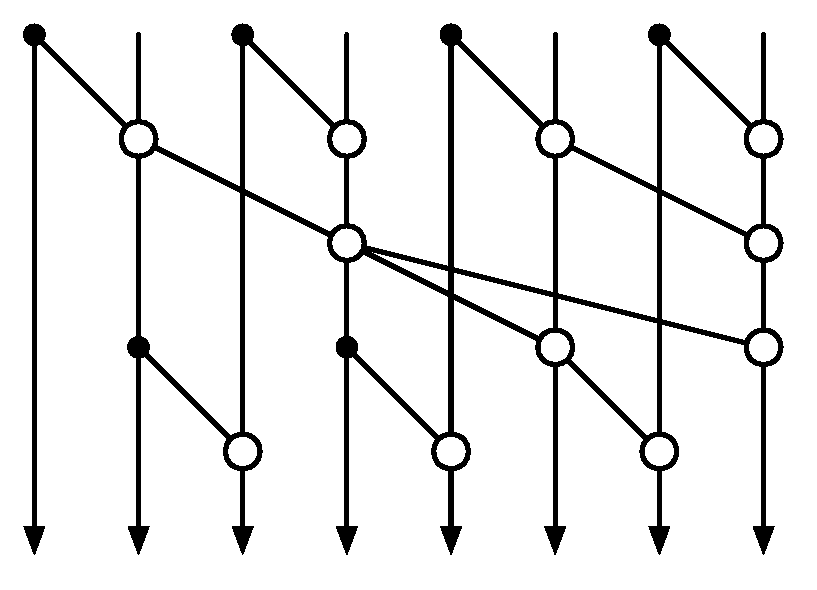
\includegraphics[scale=0.4]{scan_circuit.pdf}
  \caption{Depth-optimal scan circuit}
  \label{fig:scan-circuit}
\end{minipage}%
\begin{minipage}{.5\textwidth}
  \centering
  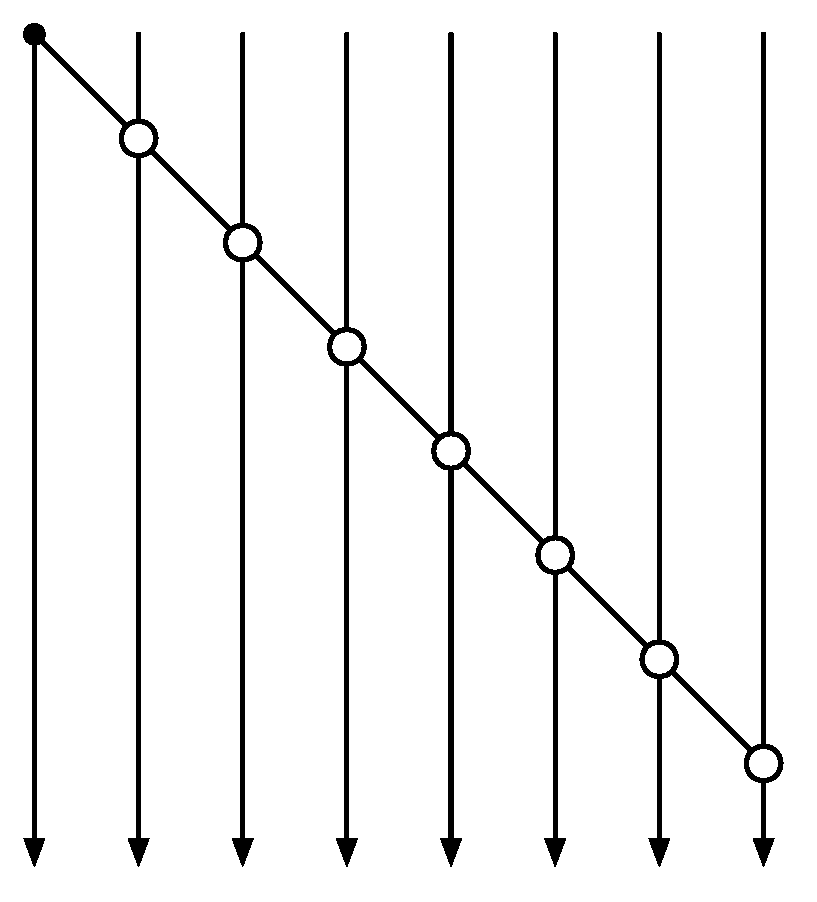
\includegraphics[scale=0.4]{scan_circuit_serial.pdf}
  \caption{Serial scan circuit}
  \label{fig:scan-circuit-serial}
\end{minipage}
% \caption{Two scan circuits of size 8}
\end{figure}

% \begin{figure}[ht]
% \centering
% 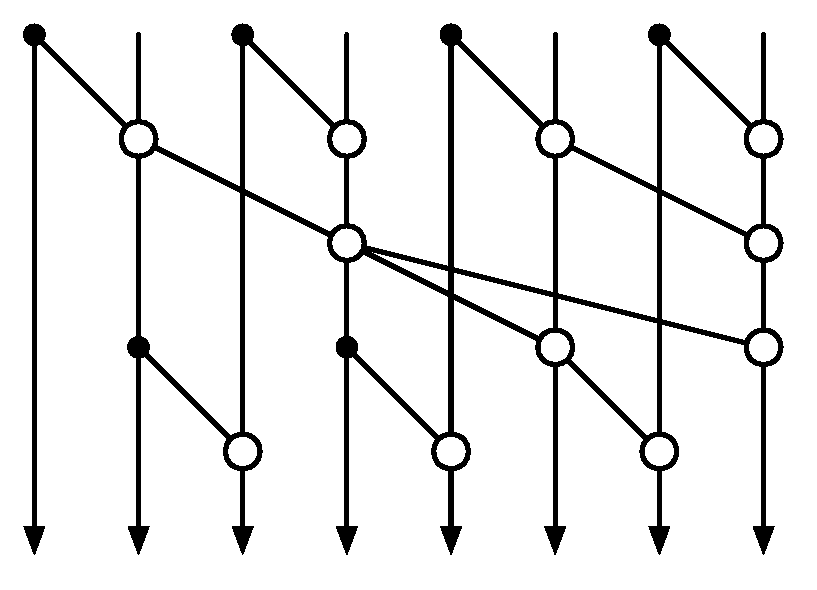
\includegraphics[scale=0.4]{scan_circuit.pdf}
% \caption{A scan circuit of size 8}
% \label{fig:scan-circuit}
% \end{figure}

Values flow from top to bottom.
At the top are the inputs, at the bottom are outputs.
The circles are operation nodes where the $\oplus$ operator is
applied.
For any number of inputs, different circuits can exist which implement
a scan.

In An algebra of scans\cite{hinze04}, Ralf Hinze describes how a
scan circuit can be constructed from smaller components using tools
like fans, stretching, horizontal (parallel) composition and vertical
composition (sequencing).
The horizontal and vertical composition are also native constructions
in Π-ware.

In particular, Hinze builds a few \emph{scan combinators}.
These are operators which combine two circuits into a bigger one, with
the extra property that if both of the arguments are scan circuits,
the result is also a scan circuit.

\section{The project}\label{The-project}

This work was done as part of an experimentation project for 15 ECTS.
The main goal was to provide a case study for Π-Ware, to see if it can
be applied to implement the algebra of scans.

This report documents what we have learned during the project.
While the biggest deliverable is the code itself, this report provides
a rationale for some of the choices and serves as documentation for
the delivered code.

\section{Additions to Π-Ware}\label{additions-to-piware}

\subsection{Combinationality}\label{combinationality}

Before this project started, the circuit data type \AD{ℂ} looked
something like this:

\InsertCode{circuit-old}

The two indices of the data type are the input and output
size.
\AI{Gate} is used to create circuits which execute functions.
\AI{Plug} is used to make circuits which just do rewiring, mapping
each output to one of the inputs.
\AI{⟫} and \AI{∥} are vertical and horizontal composition respectively.

\emph{Purely combinational} circuits have no internal state and can be
simulated without regarding past inputs.
Only the constructors \AI{Gate}, \AI{Plug}, \AI{⟫} and \AI{∥} are
necessary to create purely combinational circuits.
Scan circuits are purely combinational too.

The last constructor, \AI{DelayLoop}, is the only way to create
non-combinational circuits.
The circuit passed to \AI{DelayLoop} must however be purely
combinational.
To enforce this it takes a parameter \AB{p} \AY{:} \AF{comb} \AB{c}
which is a predicate telling whether a circuit is \emph{purely
  combinational}.

There are some practical issues with this way of handling
combinationality.
It is often annoying to have to pass the \AF{comb} proof separately,
and in case splits on \AD{ℂ} you always need a case for \AI{DelayLoop}
even when there is a \AF{comb} proof for that circuit.

But most importantly, the proof of combinationality can not be
automatically derived in many cases.
There were some functions which created some big circuits, and
separate proofs were needed to show that they were combinational.

\subsubsection{combinationality in the
  type}\label{combinationality-in-the-type}

We made two important observations:

\begin{itemize}
\item \AF{comb} \emph{restricts which circuits can be constructed},
  just like the input and output size.
\item Combinationality is something which you \emph{require} for
  certain functions, but you usually don't need to calculate whether a
  circuit is combinational.
\end{itemize}

These observations prompted the new definition of circuits, where
\AB{p} \AY{:} \AD{CombSeq} is now an index of the data type.

\InsertCode{circuit}

Reading the type of \AI{\_⟫\_}, we see that if the output circuit is
required to be combinational both arguments must be combinational, and
if the output circuit is allowed to be sequential the arguments are
allowed to be sequential too.

For \AI{DelayLoop}, the output circuit \emph{must} be allowed to be
sequential and the input circuit is required to be combinational.

This solution solves all the practical issues mentioned previously.

The approach is similar to what Conor McBride does in How to Keep
Your Neighbours in Order\cite{mcbride14}.

\subsection{Equality}\label{equality}

Many properties we want to prove are about \emph{equal behavior} of
circuits. More formally, when you simulate two circuits they are equal
if they give the same result for every possible input. We require some
properties, the first three are needed to be an equivalence
relationship:

\begin{itemize}
\item E1. Reflexivity, any circuit is equal to itself.
\item E2. Symmetry, if \AB{f} is equal to \AB{g} then \AB{g} is equal
  to \AB{f}.
\item E3. Transitivity, if \AB{f} is equal to \AB{g} and \AB{g} is
  equal to \AB{h} then \AB{f} is equal to \AB{h}.
\item E4. Circuits can be equal if their sizes are not definitionally
  the same.
For example in the property \AB{f} \AI{∥} \AF{id⤨} \AN{0} \AD{≋}
\AB{f}, where \AF{id⤨} \AB{n} is the identity circuit with size \AB{n}.
The left hand side is of size \AB{f} \AF{+} \AN{0}, but the right hand
side has size \AB{f}.
From the equality we should be able to obtain proofs that the sizes do
match.
\end{itemize}

\subsubsection{First try}\label{first-try}

A straightforward definition might be:

\InsertCode{eq1}

To prove that two circuits are equal we must build a function which
takes some input vector \AB{w} of length \AB{i}, and returns a
proof that both circuits give the same result when we simulate them with
that input. With this definition we get properties E1-3, but not E4.
Both circuits use the same variables for their sizes, input size
\AB{i} and output size \AB{o}.

\subsubsection{Semi-heterogeneous
equality}\label{semi-heterogeneous-equality}

To get property E4 we need seperate variables for the sizes of the two
circuits. This separation gives us two problems:

\begin{itemize}
\item
  The input sizes don't match, so we can't pick an input vector which
  fits both.
\item
  The output sizes don't match so the types of the result are different.
  In Agda, the propositional equality \AD{≡} is homogeneous so it
  can't be used to compare the results.
\end{itemize}

One of the solutions we tried is to coerce one of the circuits so the
sizes line up using a function of type \AY{∀} \AY{\{}\AB{i₁} \AB{i₂}
\AB{o₁} \AB{o₂}\AY{\}} \AY{→} \AB{i₁} \AD{≡} \AB{i₂} \AY{→} \AB{o₁}
\AD{≡} \AB{o₂} \AY{→} \AD{ℂ} \AB{i₁} \AB{o₁} \AY{→} \AD{ℂ} \AB{i₂}
\AB{o₂}.
This works reasonably well, but the asymmetry in the definition feels
awkward.
A prettier solution is to not use propositional equality on the
vectors.
The standard library provides a semi-heterogeneous vector
equality \AF{≈ᵥ} where the lengths of the vectors don't have to be
the same. From a proof that two vectors are equal in this way,
\AB{xs} \AF{≈ᵥ} \AB{ys}, we can obtain a proof that the lengths of the two
vectors are equal.
When you are lucky you can rewrite your goals with this proof, then
the lengths of the vectors become equal and you can convert the
semi-heterogenous equality to a propositional equality \AB{xs} \AD{≡}
\AB{ys}.
Using the semi-heterogeneous vector equality we arrive at the
following definition:

\InsertCode{eq-e}

This gives us property E4 quite elegantly.
Reflexivity (E1) and symmetry (E2) are still easy to prove.

\subsubsection{Empty domains}\label{empty-domains}

With this definition \AF{≊} we got stuck in finding a proof for
transitivity (E3).
It took a while to find the root of this problem.

The essence is that if we have two circuits \AB{f} and \AB{g}
with truly different sizes (contrary to definitionally different but
equal sizes like \AB{n} \AF{+} \AN{0} and \AB{n}), the type
\AB{w₁} \AF{≈ᵥ} \AB{w₂} becomes empty.
In that case we can always create a function which has the right
return type \AF{⟦} \AB{f} \AF{⟧}
\AB{w₁} \AF{≈ᵥ} \AF{⟦} \AB{g}
\AF{⟧} \AB{w₂}, because it will never actually
have to return anything.
Here is a proof that the identity circuit of size \AN{0} is equal to
the identity circuit of size \AN{1} (it should not be):

\InsertCode{eq-e-inconsistent}

To solve this problem, we need to make sure that the domain can never
be empty.
The standard solution to do such a thing is to combine the function
with a witness; some value of the correct type which is not really
used, but it shows that the type is not empty.
In our situation it is more fitting to require a proof that \AB{i₁}
\AF{≡} \AB{i₂}.
This is often easier to create and is sufficient.

This results in the final definition, we wrap the previous definition
\AF{≊} in a data type with a proof for \AB{i₁} \AF{≡} \AB{i₂}.

\InsertCode{eq}

Now we have all the desired properties E1 to E4.

Note: We do not have to pass \AB{o₁} \AF{≡} \AB{o₂}, but we can create
that proof in a roundabout way by creating a dummy input and passing
it to the function.
The resulting vector equality implies that the output sizes must be
equal.

\subsection{Compositionality}\label{compositionality}

The behavior of a circuit is determined by the behavior of the parts. We
can substitute any part of a circuit by another part with the same
behavior, while the whole circuit keeps the same behavior.

\subsubsection{Congruence under X}\label{congruence-under-x}

This notion was inmplemented by defining separate
\AF{X-cong}-functions for a lot of functions which combine or return
circuits. A function \AF{X-cong} tells us that \AF{X} \emph{preserves}
behavioral equality.

\InsertCode{seq-and-par-cong}

This pattern is also useful if you want to pass other kinds of
equivalences like propositional equality or vector equality:

\InsertCode{scan-and-stretch-cong}

\subsubsection{Contexts}\label{contexts}

An earlier approach was inspired by \InsertCodeInline{congTy}.

To translate this function to circuits, we use contexts instead of the
function \AF{f}.
A context is similar to a circuit, but one single hole in it
(basically half of a Huet zipper).
A circuit in the hole can be plugged with \InsertCodeInline{plugCxtTy}.
Now we can define a function similar to \AF{cong}:

\InsertCode{eq-cong}

A disadvantage of this particular definition is that the sizes of
\AB{f} and \AB{g} must be definitionally equal.
We want to be able to give \AB{f} and \AB{g} definitionally different
sizes.
A context only works on circuits of one particular size, so we need
a context for both \AB{f} and \AB{g}, and both must do the same thing
(they are equal in a certain sense).
Then we can plug one of the contexts with \AB{f} and the other with
\AB{g}.
If our context equality is \AD{≈ₓ}, we can define:

\InsertCode{eq-cong2}

With some convenient constructors for the context equality \AD{≈ₓ}
we can use it like this:

\InsertCode{cong2-example}

% \subsubsection{\texorpdfstring{Comparison of \texttt{X-cong} and
% contexts}{Comparison of X-cong and contexts}}\label{comparison-of-x-cong-and-contexts}
\subsubsection{\texorpdfstring{Comparison of \AF{X-cong} and contexts}{Comparison of X-cong and contexts}}\label{comparison-of-x-cong-and-contexts}

Compare the terms using \AF{≋-cong} and \AF{X-cong}:

\InsertCode{cong2-example-impl}

\InsertCode{x-cong-example-impl}

The \AF{X-cong}-functions have some advantages:

\begin{itemize}
\item They follow the actual structure of the circuits more closely,
  which make them easier to use.
\item It is possible to substitute both sides of an operator at the
  same time.
  This is not only shorter, but can circumvent problems when the sizes
  of the circuits are changed.
\item They extend well to other user-made constructions, while the
  contexts are only defined on the native constructors of ℂ.
\end{itemize}


\subsection{Basic properties}\label{basic-properties}

We proved a lot of basic structural properties mostly based on the
structural laws of Hinze′s scan algebra.
These include left identity, right identity and associativity of
\AD{⟫} and \AD{∥}, distributivity of \AD{∥} over \AD{⟫} and merging of
parallel \AF{id⤨}'s.

\subsection{Plugs}\label{plugs}

At the start of the project, plugs in Π-Ware were defined using
rewiring function of type \AF{fin} \AB{o} \AY{→} \AF{fin} \AB{i}.
For any output wire, this function tells you which input wire it is
connected to.
The evaluation of a plug was basically \AF{⟦} \AI{Plug} \AB{p} \AF{⟧}
\AB{w} \AY{=} \AF{tabulate} \AY{(λ} \AB{n} \AY{→} \AF{lookup}
\AY{(}\AF{p} \AB{n}\AY{)} \AB{w}\AY{)}.
Doing proofs with this higher order representation can get quite
complicated, because the function is used as a higher order argument
within the \AF{tabulate} and \AF{lookup}.

Later the plugs changed to a first-order representation \AD{Vec}
\AY{(}\AD{Fin} \AB{i}\AY{)} \AB{o}.
This makes them a bit easier to reason about, but it does not make the
evaluation simpler - actually, it adds a \AF{lookup}.

\subsubsection{Plugs by morphism}\label{plugs-by-morphism}

To alleviate this problem, we use \AD{Vec-Morphism}:

\InsertCode{vec-morphism}

And we can build plugs, in the current system, using these morphisms:

\InsertCode{plug-by-morphism}

The fact that \AL{op} is \emph{parametrically polymorphic} guarantees
that it commutes with map, as is shown in Theorems for free! by Philip
Wadler.
However, we can not get this theorem for free in Agda, so we need
\AL{op-map-commute} to be in the record.
Using \AL{op-map-commute}, we can prove a simple but powerful
property:

\InsertCode{plug-by-morphism-is-cool}

We just got rid of all the \AF{tabulate}'s and \AF{lookup}'s! This
makes a lot of proofs simpler.

\section{Patterns}\label{patterns}

When we use a function to generate some kind of circuit, we call it a
pattern.
Patterns usually have a few things in common, taking the \AF{fan}
pattern as an example:

\begin{itemize}
\item
  The pattern function: \InsertCodeInline{fan-ty}
\item
  An implementation: \InsertCodeInline{fan-impl-ty}
\item
  A specification: \InsertCodeInline{fan-spec-ty}
\item
  Proof that the pattern function matches the implementation:
  \InsertCodeInline{reveal-fan-ty}
\item
  Proof that the implementation matches the specification:
  \InsertCodeInline{fan-to-spec-ty}
\end{itemize}

The reason for separating the pattern function and implementation is
that we often mark the pattern function as abstract, so it wont reduce
when we don't want it too.
This is a good way to hide the complexity of patterns.
We often do not need to know the actual implementation to be able to
use them, so we can start viewing the problem at hand from a higher
level of abstraction.
In some cases it also leads to better performance.

For future work, it might be useful to make this structure more
formal.
During simulation this might be particularly useful, because you could
choose to run the specification instead of simulating the
implementation circuit.
This might make simulation of very large circuits feasible.

\subsection{Heterogeneous sequencing}\label{heterogeneous-sequencing}

To put two circuits in sequence with the native \AI{\_⟫\_}
constructor, the sizes must be the same.
To be able to put two circuits in sequence where the output size of
the first is not the same, but known to be equal, to the input size of
the second, the following \emph{heterogeneous sequencing} pattern is
defined:

\InsertCode{hetseq-ty}

Together with a variant where the proof is implicit:

\InsertCode{hetseq-implicit-ty}

It is used like this:

\InsertCode{hetseq-proof-example}

This is a great example where marking the pattern function as abstract
is very useful:
When \AB{m} and \AB{n} are the same, Agda reduces the implementation
so far that it does not recognize it as a \AF{\_⟫[]\_} anymore.
Without marking the pattern function as abstract, it might happen that
a function which can be applied to \AB{f} \AP{⟫[} \AB{p} \AP{]} \AB{g}
can not be applied to \AB{f} \AP{⟫[} \AF{refl} \AP{]} \AB{g}.

% \subsubsection{\texorpdfstring{\texttt{⟫{[}{]}-cong}}{⟫{[}{]}-cong}}\label{cong}

\subsubsection{\texorpdfstring{Congruence under
    \AF{⟫[]-cong}}{Congruence under ⟫[]-cong}}\label{cong}

Something similar to \AF{⟫-cong} can be defined for heterogeneous
sequencing \AF{⟫[]}:

\InsertCode{hetseq-cong}

Also, it can be useful to quickly convert from \AF{⟫} to \AF{⟫[]}, and
back if the sizes allow it.
Besides some simple conversion functions we can define two variants of
\AF{⟫[]-cong}:

\InsertCode{hetseq-cong-tofrom}

Notice that the convention here is that the proofs for the left hand
side are given by the user, and the proofs on the right hand side are
provided by the function.
This convention makes it possible to automatically create the equality
proofs in a lot of cases, for example:

\InsertCode{hetseq-proof-example}

This convention is also followed by many of the properties regarding
heterogeneous sequencing.
The drawback of this is that it breaks when the proof is flipped with
\AF{≋-sym}, resulting in forwards and backwards variants of some of
the properties.

\subsection{Stretching}\label{stretching}

The stretch operator \AF{⤙} is straight from Hinze's paper and can
be used to stretch a circuit by a list of widths $a_1,\ a_2,\ ...,\
a_n$ where \AF{n} is both the input and output size of the circuit.
From the standpoint of the resulting circuit, its inputs and outputs
are grouped such that every group \AB{i} has length \AB{aᵢ}.
For each \AB{i}th group, the first in-/output is connected to the
\AF{i}th wire of the inner circuit.
We can implement it by first reordering the wires, passing the first
\AF{n} of them through the inner circuit and then reversing the
original reordering:

\InsertCode{stretch}

Where \AF{size} \AB{m} \AB{as} = \AF{sum} \AY{(} \AF{map} \AY{(}
\AF{\_+\_} \AB{m} \AY{)} \AB{as} \AY{)}.

The hard part is to come up with a definition for \AF{in-⤨} and
\AF{out-⤨} such that it is easy to do proofs about them.

\subsubsection{Permutations}\label{permutations}

Initially we wanted to work with the fact that both \AF{⟦} \AF{in-⤨}
\AF{⟧} and \AF{⟦} \AF{out-⤨} \AF{⟧} must return a permutation of their
input.

We formalized this using Lehmer codes, a way of uniquely encoding
permutations.
We did proofs about these Lehmer codes about their composibility,
inversion, identities and application to vectors.

This method works fine if you want, for instance, the property that
\InsertCodeInline{in-out-id-ty}.
It breaks down when you want to reason about where certain elements go
and what is done to them, so we decided not to use it.
We replaced it by plugs by morphism, as described in section
\ref{plugs-by-morphism}.

\subsubsection{MinGroups}\label{mingroups}

The current version uses an explicit representation of groups.
The data type \AD{MinGroups} \AB{A} \AB{m} \AB{as}, is basically a
vector of vectors.
If \AB{as} is a list $a_1,\ a_2,\ ...,\ a_n$, the \AB{i}th vector is
of size \AB{m} \AF{+} \AB{aᵢ}.
We can convert a vector of the right size to a \AD{MinGroups} and
back, essentially splitting a vector into groups.
We define a function \InsertCodeInline{extract-map-ty}, which performs
the following steps:

\begin{enumerate}
\item Take the first element of each group and put them in a vector.
\item Apply a function to this vector.
\item Insert the elements of the resulting vector as the first element of
  each group.
\end{enumerate}

This \AF{extract-map} has some nice properties like composability and
that it commutes with concatenation.
There are several properties about \AD{MinGroups} and \AF{extract-map}
which are obvious but still hard to prove, a few of those are simply
postulated.

\subsubsection{More stretching}\label{more-stretching}

We also define a \AF{⤚} operator, which is the same as \AF{⤙} except
that it works on the last element of each group instead of the first.
Many proofs about stretches are defined such that they work on both
directions.
There are also derived stretch operators \AF{⤜} and \AF{⤛}, which use
a list of circuits instead of the list of widths.
They inherit most of the properties of the basic stretch operators.

\subsection{Fans}\label{fans}

\begin{figure}[ht]
\centering
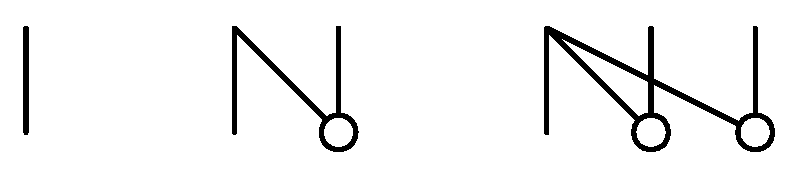
\includegraphics[scale=0.25]{fans_123.pdf}
\caption{Fans of sizes 1, 2 and 3}
\label{fig:fans}
\end{figure}

In Ralf Hinze's scan algebra, fans are native constructions.
Given some inputs $x_1,\ x_2,\ \ldots{},\ x_n$, the circuit \AF{fan}
\AB{n} has outputs $x_1,\ (x_1\ \oplus\ x_2),\ (x_1\ \oplus\ x_3),\
\ldots{},\ (x_1\ \oplus\ x_n)$ (figure \ref{fig:fans}).

In Π-Ware, fans have to be defined using smaller circuits.
We can build a \AF{plusℂ} circuit with two inputs and one output which
applies the $\oplus$ operator, using the \AI{Gate} constructor of \AD{ℂ}.

\begin{figure}[ht]
\centering
\begin{minipage}{.5\textwidth}
  \centering
  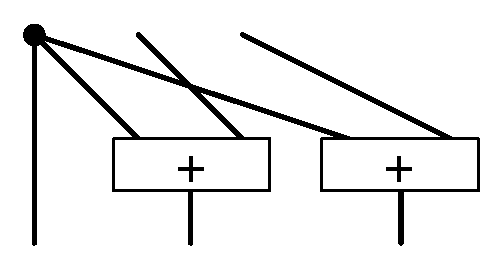
\includegraphics[scale=0.4]{fan_structure_old.pdf}
\end{minipage}%
\begin{minipage}{.5\textwidth}
  \centering
  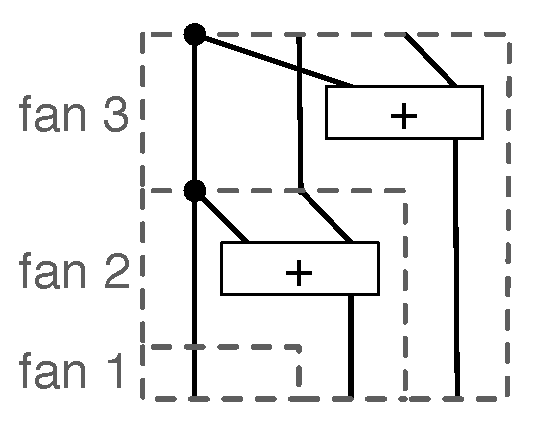
\includegraphics[scale=0.4]{fan_structure.pdf}
\end{minipage}
\caption{Structure of fans. Left: first approach, right: current approach}
\label{fig:fan-structure}
\end{figure}

At first, we defined \AF{fan}s as a \AI{Plug} followed by a bunch of
\AF{plusℂ}'s in parallel (figure \ref{fig:fan-structure}, left).
The definition itself is quite easy and elegant, but it was very hard
to prove things about because there is no structure to recurse on.

In the current version we built them iteratively, using smaller fans
to make the bigger ones (figure \ref{fig:fan-structure}, right).

% \begin{figure}[ht]
% \centering
% 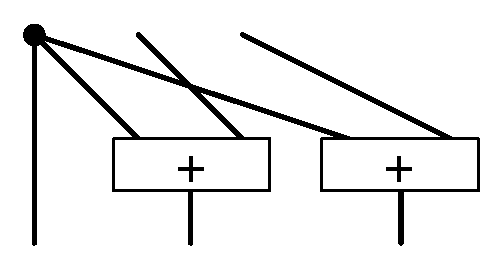
\includegraphics[scale=0.4]{fan_structure_old.pdf}
% \caption{Structure of fans}
% \label{fig:fan-structure-old}
% \end{figure}

% \begin{figure}[ht]
% \centering
% 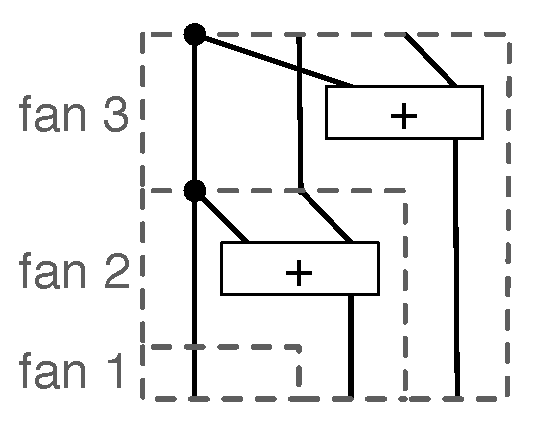
\includegraphics[scale=0.4]{fan_structure.pdf}
% \caption{Structure of fans}
% \label{fig:fan-structure}
% \end{figure}

Note: Maybe fans can also be implemented by using an indexed variant
of the \AI{Gate} constructor, but this was not researched thoroughly.

\subsection{Scans}\label{scans-1}

\begin{figure}[ht]
\centering
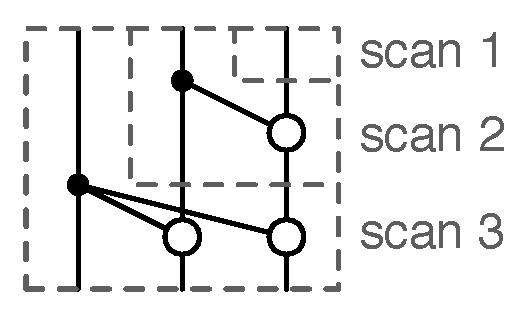
\includegraphics[scale=0.4]{scan_structure.pdf}
\caption{Structure of naive scans}
\label{fig:scan-structure}
\end{figure}

When we have a scan circuit of size \AB{n}, we can create a scan
circuit of size \AB{n} \AF{+} \AN{1} by using \AF{scan-succ}.

\InsertCode{scan-succ}

From this definition we can derive a very simple method to create scan
circuits of any size, as in figure \ref{fig:scan-structure}:

\InsertCode{scan}

This is the least efficient scan possible, both in depth and the
number of operation nodes.
It is, however, quite easy to work with.

Now we can make the statement ``*something* is a scan circuit'' more
formal:
Given a circuit \AB{f} \AY{:} \AD{ℂ} \AB{n} \AB{n}, we can say that
\AB{f} \emph{is a scan circuit} if we have a proof that \AB{f} \AF{≋}
\AF{scan} \AB{n}.

\subsubsection{Scan combinators}

Two of the scan combinators defined by Hinze are the vertical scan
combinator \AF{▱} and horizontal scan combinator \AF{⌷}:

\InsertCode{scan-combinators}

We were able to prove for both combinators that if we use them to
combine two scans, we get another scan:

\InsertCode{scan-combinator-proofs}

\subsubsection{Serial scans are scans}

With all these tools we can do proofs about real scans.
Take for instance the \emph{serial scan}.
This is a scan where all operations are done in sequence, see figure
\ref{fig:scan-circuit-serial}.
It is the normal way to implement a scan without using parallelism.

Here we use \AF{id⤨} and \AF{\_⟫[\_]\_} to make the size of \AF{serial-scan}
\AY{(}\AI{suc} \AB{n}\AY{)} \AF{⌷} \AF{id⤨} \AN{1} line up with the
type.

\InsertCode{serial-scan}

Like many scans, serial scans are built from smaller scans using scan
combinators.

To prove that a serial scan is indeed a scan circuit (is equal to
\AF{scan} \AB{n}), we simply have to prove that the parts are scans.
In this case that is done by induction and with the fact that
\AF{id⤨} \AN{1} \AF{≋} \AF{scan} \AN{1}.
When we have proved that the components are scans, we know that the
whole circuit is a scan too. Here is a full proof:

\InsertCode{serial-scan-is-scan}

\section{Future work}\label{future-work}

One example where the system does not work as easy as we would like,
is in proving that \AF{scan-succ} \AY{(}\AB{f} \AF{▱} \AF{scan-succ}
\AB{g} \AF{⟫[} \AB{p} \AF{]} \AF{id⤨}\AY{)} \AD{≋} \AF{scan-succ}
\AB{f} \AF{▱} \AF{scan-succ} \AB{g}.
Where Hinze uses 9 lines, we need 110 (!) lines.
This is mainly because we need to prove a lot of boring things like
\AB{a} \AF{⟫} \AB{b} \AF{⟫} (\AB{c} \AF{⟫} \AB{d}) \AD{≋} \AB{a}
\AF{⟫} (\AB{b} \AF{⟫} \AB{c}) \AF{⟫} \AB{d}.
It would be nice to have some kind of automated way of building
proofs similar to the semiringsolver in the standard library.
This might be done by normalizing circuits with \AI{⟫}, \AI{∥},
\AF{id⤨} and \AI{⟫[]} to some normal form.

Some things are still postulated, and should be proven formally.
Most of these are quite 'obviously' true, or are a free theorem (see
section \ref{plugs-by-morphism}.

\section{Conclusion}\label{conclusion}

We have shown that we can prove properties about whole families of
circuits.
These proofs can be written quite intuitively with equational
reasoning.
Many proofs follow exactly the same structure as Hinze's proofs.

In the course of this project, we have built several patterns (section
\ref{patterns}) on top of Π-Ware.
We have shown that it is possible to work with a high-level pattern
like scan, without really noticing that they are actually composed of
other things like fans and plugs.

Besides some left-over postulates, we have formally proven that certain
circuits are scans, and that scans can be combined to create other
scans.
